%% UzK - A BEAMER THEME FOR THE UNIVERSITY OF COLOGNE
%% http://solstice.github.com/uzk-theme/

\documentclass{beamer}
%\usefonttheme{serif}
\usefonttheme{professionalfonts}%  don't change fonts inside beamer
%\usepackage[ngerman]{babel}
%\usepackage[latin1]{inputenc}
%\usepackage[T1]{fontenc}
\usepackage{polyglossia}
\setmainlanguage{english}
\usepackage{fontspec}
\usepackage{xeCJK}
\usepackage{unicode-math}
	\setmathfont{Latin Modern Math} % default
	%\setmathfont[range=\mathalpha]{Asana Math}
	%\setmathfont{Asana Math}[range={\mathbin}] %\mathord
	\setmathfont{STIX Math}[range={"02609}] % ☉
	%\setmathfont{Latin Modern Math}[range={"1D608-"1D63B}, sans-style=italic]
	%\setmathfont{Latin Modern Math}[range={"00391-"003A9, "003B1-"003F5}, sans-style=upright]
\usepackage{siunitx}

%% Falls Anzeige der \sections, \subsections etc. gewuenscht, kann zB.
%% das infolines theme geladen werden. Wichtig ist jedoch, dass andere
%% Themes _vor_ dem UzK-Theme geladen werden.
%\useoutertheme{infolines}

%% Falls keine der Optionen zur Bestimmung der Fusszeile uebergeben werden    %%
%% werden alle Fakultaetsfarben verwendet. ---------------------------------- %%
\usetheme[%
%wiso,        %% Wiso-Fakultaet
%jura,        %% Rechtswissenschaftliche Fakultaet
%medizin,     %% Medizinische Fakultaet
%philo,       %% Philosophische Fakultaet
%matnat,      %% Mathematisch-Naturwissenschaftliche Fakultaet
%human,       %% Humanwissenschaftliche Fakultaet
%verw,        %% Universitaetsverwaltung
%nav,         %% Schaltet die Navigationssymbole ein
latexfonts,  %% Verwendet die latex-beamer-Standardschrift
%colorful,    %% Farbige Balken im infolines-Theme
%squares,     %% Aufzaehlungspunkte rechteckig
%nologo,      %% Kein Logo im Seitenhintergrund
]{UzK}

%\title{Beamer-Theme \texttt{UzK} für Präsentationen im Corporate
%  Design der Universität zu Köln}
  \title%[Short Paper Title] % (optional, use only with long paper titles)
{Black Hole Thermodynamics}
\subtitle{And Hawking Radiation}

\author[Arenas, Schmitz, Wang] % (optional, use only with lots of authors)
{Sebastiàn Arenas \and Tim Schmitz \and Yi-Fan Wang 王一帆}

\date{Advanced Seminar on Relativity and Cosmology}

%\author[David Kusterer \and Bernd Weiß]%
%{David Kusterer\thanks{ \href{mailto:kusterer@uni-koeln.de}{kusterer@uni-koeln.de} }%
%  \and%
%  Bernd Weiß\thanks{\href{mailto:bernd.weiss@wiso.uni-koeln.de}{bernd.weiss@wiso.uni-koeln.de}}}

%\institute[Forschungsinstitut für Soziologie]{%
%Forschungsinstitut für Soziologie \\
%Greinstraße 2\\
%50939 Köln}
%\institute[Uni Köln]{Universität zu Köln}

\usepackage[citestyle=alphabetic,doi=false,isbn=false,url=false]%
	{biblatex}
\addbibresource{black-holes.bib}

\usepackage{tikz}
\usetikzlibrary{decorations.pathmorphing}
\usetikzlibrary{calc}

\usepackage{cleveref}

\usepackage{braket}


% Math symbols and user-defined extensions


% some unicode characters
% ≙ for equal with hat


% Mathematical constants
\newcommand{\ii}{{\Bbbi}}
\newcommand{\ee}{{\Bbbe}}
\newcommand{\pp}{{\Bbbpi}}

% Bracket-like
\newcommand{\rbr}[1]{{\left(#1\right)}}
\newcommand{\sbr}[1]{{\left[#1\right]}}
\newcommand{\cbr}[1]{{\left\{#1\right\}}}
\newcommand{\abr}[1]{{\left<#1\right>}}
\newcommand{\vbr}[1]{{\left|#1\right|}}
\newcommand{\fat}[2]{{\left.#1\right|_{#2}}}
% Functions; note the space between the name and the bracket!
\newcommand{\rfun}[2]{{#1}\mathopen{}\left(#2\right)\mathclose{}}
\newcommand{\sfun}[2]{{#1}\mathopen{}\left[#2\right]\mathclose{}}
\newcommand{\cfun}[2]{{#1}\mathopen{}\left\{#2\right\}\mathclose{}}
\newcommand{\afun}[2]{{#1}\mathopen{}\left<#2\right>\mathclose{}}
\newcommand{\vfun}[2]{{#1}\mathopen{}\left|#2\right|\mathclose{}}
% Differentials
\newcommand{\Dif}{\BbbD}
\newcommand{\Diff}{\,\BbbD}
\newcommand{\dif}{\Bbbd}
\newcommand{\diff}{\,\Bbbd}
\newcommand{\dva}{\mupdelta} % no better way?!
\newcommand{\dvar}{\,\mupdelta}
% Fraction-like
\newcommand{\frde}[2]{{\frac{\dif{#1}}{\dif{#2}}}}
\newcommand{\frDe}[2]{{\frac{\Dif{#1}}{\Dif{#2}}}}
\newcommand{\frpa}[2]{{\frac{\partial{#1}}{\partial{#2}}}}
% Equal marks
\newcommand{\eeq}{{\overset{!}{=}}}
\newcommand{\lls}{{\overset{!}{<}}}
\newcommand{\ggt}{{\overset{!}{>}}}
\newcommand{\lle}{{\overset{!}{\le}}}
\newcommand{\gge}{{\overset{!}{\ge}}}
% overline-like marks
\newcommand{\ol}[1]{{\overline{{#1}}}}
\newcommand{\ul}[1]{{\underline{{#1}}}}
\newcommand{\tld}[1]{{\widetilde{{#1}}}}
\newcommand{\ora}[1]{{\overrightarrow{#1}}}
\newcommand{\ola}[1]{{\overleftarrow{#1}}}
\newcommand{\td}[1]{{\widetilde{#1}}}
\newcommand{\what}[1]{{\widehat{#1}}}
%\newcommand{\prm}{{\symbol{"2032}}}

% Math operators
% Why does \DeclareMathOperator not work?
\DeclareMathOperator{\sgn}{sgn}
\DeclareMathOperator{\grad}{grad}
\DeclareMathOperator{\curl}{curl}
\DeclareMathOperator{\rot}{rot}
\DeclareMathOperator{\opdiv}{div}
\DeclareMathOperator{\opdeg}{deg}

\DeclareMathOperator{\sech}{sech}
\DeclareMathOperator{\csch}{csch}

\DeclareMathOperator{\diag}{diag}
\DeclareMathOperator{\tr}{tr}

\DeclareMathOperator{\ad}{ad}

\DeclareMathOperator{\expi}{expi}

% Group and Algebras
\newcommand{\SO}{\mathsf{SO}\,}
\newcommand{\SU}{\mathsf{SU}\,}
\newcommand{\so}{\mathfrak{so}\,}
\newcommand{\su}{\mathfrak{su}\,}


\begin{document}

\begin{frame}%[titlepage]
  \titlepage
\end{frame}

\begin{frame}{Outline}
%  \tableofcontents
  % You might wish to add the option [pausesections]
\begin{enumerate}
\item {\makebox[4cm][l]{Introduction} Tim}
\item {Laws of black hole mechanics and thermodynamics}
	\begin{enumerate}
	\setcounter{enumii}{-1}
	\item {\makebox[3cm][l]{The \alert{second} law} Tim}
	\item {\makebox[3cm][l]{The \alert{zeroth} law} Sebastiàn}
	\item {\makebox[3cm][l]{The \alert{first} law} Sebastiàn}
	\item {\makebox[3cm][l]{The third law} Sebastiàn}
	\end{enumerate}
\item {\makebox[4cm][l]{Hawking radiation} Yi-Fan}
\end{enumerate}
\end{frame}

\begin{frame}{Outline}
  \tableofcontents
  % You might wish to add the option [pausesections]
\end{frame}

\section{Motivations}

\begin{frame}{Motivations for the Radiation}%
{Developments in classical physics}
\begin{itemize}
\item (Speculative) entropy and temperature of black holes
	\cite{Bekenstein1973,Bekenstein1980}
\item Penrose process and super-radiance
\end{itemize}

\end{frame}

\begin{frame}{Motivations for the Radiation}%
{Developments in quantum physics}

\begin{itemize}
\item Arguments from fundamental principles
	\begin{itemize}
	\item Uncertainty principle (black holes ``might split up''
		\cite{susskind2008black})
	\item Vacuum polarisation (e.g.\ Schwinger Effect, where electron-positron
	pairs are pulled out from vacuum in strong external electric field), see
	e.g.\ \cite{Frolov1998}
	\end{itemize}

\item Arguments from field theory in curved space-time:
definition of particle ambiguous \cite{Fulling1973}, leading to particle
creations
	\begin{itemize}
	\item in dynamical universes, see e.g.\ \cite{parker2009quantum}
	\item for accelerated observers \cite{Fulling1973,Davies1975,Unruh1976}
	\end{itemize}
\end{itemize}

\end{frame}


\section{Particle creation in curved space-time}

\begin{frame}{Scalar Field in Special Relativity}{Warm-up}
\begin{itemize}
\item Diagonalising Hamiltonian: \emph{Fourier} kernel \& `\emph{momentum}' $p$
\[
\rfun{\tilde{\phi}}{p} \propto \int \dif x\,\ee^{-\ii p x} \rfun{\phi}{x},
\quad
\rfun{\tilde{\pi}}{p} \propto \int \dif x\,\ee^{+\ii p x} \rfun{\pi}{x}.
\]
\item Trsfing field between inertial obs.\ $A$ and $B$: Poincaré $\mscrP$
%\begin{alignat*}{3}
\begin{align*}
x &\to \mscrP x = \Lambda x + x_0,\quad p \to \mscrP p = p+p_0;
\\
\rfun{\tilde{\phi}_A}{p} &\to \rfun{\tilde{\phi}_A}{\mscrP^{-1}p}
\propto \rfun{\tilde{\phi}_B}{p'},\quad\text{etc.}
%\qquad &\rfun{\tilde{\pi}}{p} &\to \rfun{\tilde{\pi}}{\mscrP^{-1}p}.
\end{align*}
%\end{alignat*}
\item Canonical quantisation: ladder operators
\[ \rfun{\what{a}_\phi}{p} \propto
E_p^{+\frac{1}{2}}\rfun{\what{\tilde{\phi}}}{p}
+ \ii E_p^{-\frac{1}{2}}\rfun{\what{\tilde{\pi}}^\dagger}{p},
\quad \text{etc.}\]
\item Trsfing ladder optrs btw.\ inertial obs.: particle \alert{remains}
p.\
\[
\rfun{\what{b}}{p'}
= \what{U}_\mscrP\rfun{\what{a}}{p}\what{U}^\dagger_\mscrP
\propto \rfun{\what{a}}{\mscrP p},\quad\text{etc.}
\]
\end{itemize}
\end{frame}

\begin{frame}{Scalar Field in General Relativity}{The technical advance
we just mentioned}
\begin{itemize}
\item Diagonalising Hamiltonian: \emph{general} kernel \& \emph{parameter} $k$
\[
\rfun{\tilde{\phi}}{k} \propto \int \dif x\,\rfun{K}{k;x} \rfun{\phi}{x},
\quad
\rfun{\tilde{\pi}}{k} \propto \int \dif x\,\rfun{K^*}{k;x} \rfun{\pi}{x}
\]
\item Trsfing field between (time-like) obs.: general diffeom.\ $\mscrD$
%\begin{alignat*}{3}
\begin{align*}
x &\to \chi = \rfun{f}{x},\quad k \to \kappa = \rfun{g}{k};
\\
\rfun{\tilde{\phi}_A}{k} &\to \rfun{\tilde{\phi}_A}{\rfun{g^{-1}}{\kappa}}
=\int \dif \kappa\,\rfun{T}{k;\kappa}\rfun{\tilde{\phi}_B}{\kappa},
\quad \text{etc.}
%&\rfun{\tilde{\pi}}{k} &\to \rfun{\tilde{\pi}}{\rfun{g^{-1}}{\kappa}}.
\end{align*}
%\end{alignat*}
\item Canonical quantisation: ladder operators
\[ \rfun{\what{a}_\phi}{k} \propto
E_k^{+\frac{1}{2}}\rfun{\what{\tilde{\phi}}}{k}
\pm \ii E_k^{-\frac{1}{2}}\rfun{\what{\tilde{\pi}}^\dagger}{k},
\quad \text{etc.}\]
\item Transforming ladder optrs: \alert{Bogolyubov}, \alert{mixing} p.\ \& anti-p.\
\[
\rfun{\what{b}}{\kappa}
= \what{U}_\mscrD \rfun{\what{a}}{k}\what{U}^\dagger_\mscrD
\propto \int \dif k\,\rfun{\alpha}{\kappa;k} \rfun{\what{a}}{k}
+ \rfun{\beta}{\kappa;k} \rfun{\what{a}^\dagger}{k},
\quad\text{etc.}
\]
\end{itemize}
\end{frame}

\begin{frame}{Scalar Field in Special and General Relativity}{Particle
`creation'}
\begin{itemize}
\item Defining the $\what{a}$-vacuum as being annihilated by all $\hat{a}$'s
\[\rfun{\what{a}}{p\text{ or }k}\Ket{\Omega} \equiv 0\]
\item Number operators transform as
\begin{align*}
\rfun{\what{a}^\dagger}{p} \rfun{\what{a}}{p}
&\to \rfun{\what{b}^\dagger}{p'} \rfun{\what{b}}{p'}
&\phantom{}&\rfun{\what{a}^\dagger}{k} \rfun{\what{a}}{k} 
\to \rfun{\what{b}^\dagger}{\kappa} \rfun{\what{b}}{\kappa}\\
&\propto \rfun{\what{a}^\dagger}{\mscrP p} \rfun{\what{a}}{\mscrP p};
&=& \ldots \what{a}^\dagger \what{a} + \ldots \what{a} \what{a}
+ \ldots \what{a}^\dagger \what{a}^\dagger \\
&&+& \int \dif k\, \vbr{\rfun{\beta}{\kappa;k}}^2
\rfun{\what{a}}{k} \rfun{\what{a}^\dagger}{k}.
\end{align*}
\item $\abr{\what{n}_a}_\Omega$'s transform as
\begin{align*}
\abr{\rfun{\what{a}^\dagger}{p} \rfun{\what{a}}{p}}
&\to
\abr{\rfun{\what{b}^\dagger}{p'} \rfun{\what{b}}{p'}}
&
\abr{\rfun{\what{a}^\dagger}{k} \rfun{\what{a}}{k}}
&\to 
\abr{\rfun{\what{b}^\dagger}{\kappa} \rfun{\what{b}}{\kappa}}
\\
&= 0; &&= \int \dif k\, \vbr{\rfun{\beta}{\kappa;k}}^2.
\end{align*}
\end{itemize}

\end{frame}

\section{Gravitational collapse}

\begin{frame}{Spherically gravitational collapse}%
{The model and its quantisation}
\begin{columns}
\begin{column}{.61\textwidth}
\begin{itemize}
\item Massless neutral scalar field on the given background space-time w/
in- and out-going eigen-modes
\begin{align*}
f_{\omega'lm} &\propto r^{-1}F_{\omega'}\ee^{\ii\omega' v}
\rfun{Y_{lm}}{\theta,\phi}, \\
p_{\omega lm} &\propto r^{-1}P_{\omega}\ee^{\ii\omega u}
\rfun{Y_{lm}}{\theta,\phi}
\end{align*}
\item Quantising at Cauchy surfaces
\begin{enumerate}
\item Early time: $\what{a}$'s defined on $\mscrI^-$
\item Late time: $\what{b}$'s on $\mscrI^+$, $\what{c}$'s on $\mscrH^+$
\end{enumerate}
\item \emph{Physical} vacuum: $\what{a}\Ket{H} \equiv 0$
\item Concerned with $\Braket{H | \what{n}_b | H}$
\end{itemize}
\end{column}
\begin{column}[c]{.38\textwidth}
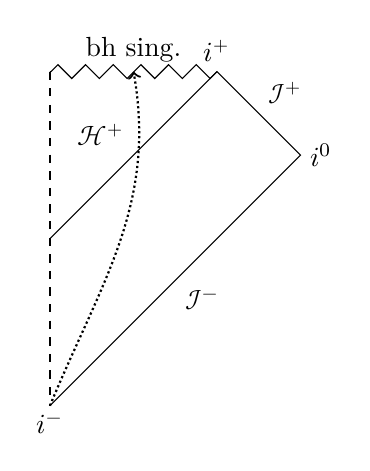
\begin{tikzpicture}%[scale=2]
\pgfmathsetmacro\myunit{3} 
\pgfmathsetmacro\sc{1.414213562} 
	\draw [dashed] (0,0)
		-- ++(-90: \sc * \myunit)
			node [below] {$i^-$}
			coordinate (a);
	\draw (a)
		-- ++(45: 1.5 * \myunit)
			node [right] {$i^0$}
			node [pos = .5, below right] {$\mscrI^-$}
		-- ++(135: 0.5 * \myunit)
			node [above] {$i^+$}
			node [pos = .5, above right] {$\mscrI^+$}
			coordinate (b)
		-- ++(-135: \myunit)
			node [pos = .5, above left] {$\mscrH^+$};
	\draw [decorate, decoration=zigzag] (b)
		-- (0,0)
			node [pos = .5, above] {bh sing.};
	\draw [densely dotted, out = 67.5, in = -80, thick, ->] (a)
			to (\sc/4* \myunit, 0);
\end{tikzpicture}
\end{column}
\end{columns}
\end{frame}

\begin{frame}{Spherically gravitational collapse}{Hawking's construction
\cite{HAWKING1974,Hawking1975}}
\begin{columns}
\begin{column}{.61\textwidth}
\begin{itemize}
\item Consider $p_\omega$ on $\mscrI^+$ propagating backwardly
to $\mscrI^-$, ending up with
	\begin{itemize}
	\item The same freq.\ $p_\omega^{(1)}$: \alert{only} gives a
	$\rfun{\delta}{\omega-\omega'}$ term in $\rfun{\alpha}{\omega;\omega'}$
	\item The rest $p_\omega^{(2)}$: contributing to $\beta$ as well;
	\alert{of interest}
	\end{itemize}
\item On $\mscrI^-$, approximately $p_\omega^{(2)} \propto$ 
\[
\begin{cases}
0, & v > v_0; \\
r^{-1}P_\omega \rbr{\frac{v_0 - v}{CD}}^{-\ii\frac{\omega}{\kappa_\text{S}}},
& v \lesssim v_0
\end{cases}
\]
where $v_0$ is the latest time a null geodesic could leave $\mscrI^-$,
$C$ and $D$ const.\
%	\begin{enumerate}
%	\item 
%	\item $\beta$ comes mainly from the high-freq.\ modes (b/c of grav.\
%	blue-shift) with $v_0-v \gtrsim 0$
%	\end{enumerate}
\end{itemize}
\end{column}
\begin{column}{.38\textwidth}
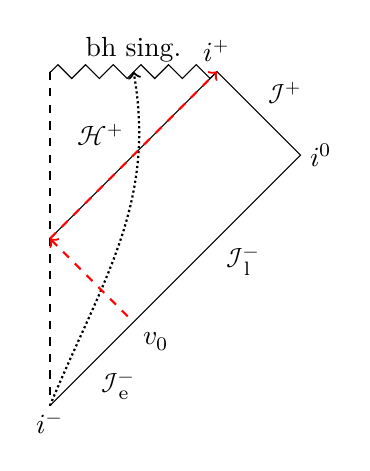
\begin{tikzpicture}%[scale=2]
\pgfmathsetmacro\myunit{3} 
\pgfmathsetmacro\sc{1.414213562} 
	\draw [dashed] (0,0)
		-- ++(-90: \sc * \myunit)
			node [below] {$i^-$}
			coordinate (a);
	\draw (a)
		-- ++(45: 1.5 * \myunit)
			node [right] {$i^0$}
			node [pos = .3333333333, below right] {$v_0$}
			node [pos = .1666666666, below right] {$\mscrI^-_\text{e}$}
			node [pos = .6666666666, below right] {$\mscrI^-_\text{l}$}
		-- ++(135: .5 * \myunit)
			node [above] {$i^+$}
			node [pos = .5, above right] {$\mscrI^+$}
			coordinate (b)
		-- ++(-135: \myunit)
			node [pos = .5, above left] {$\mscrH^+$}
			coordinate (B);
	\draw [decorate, decoration=zigzag] (b)
		-- (0,0)
			node [pos = .5, above] {bh sing.};
	\draw [densely dotted, out = 67.5, in = -80, thick, ->] (a)
			to (\sc/4* \myunit, 0);
	\draw [red, dashed, thick, <-] (B) --++(-45: .5*\myunit);
	\draw [red, dashed, thick, ->] (B) --++(+45: \myunit);
\end{tikzpicture}
\end{column}
\end{columns}
\end{frame}

\begin{frame}{Results and Interpretation}{Hawking temperature}
\begin{itemize}
\item Expectation value of particle number 
\begin{equation}
\abr{\rfun{\what{n}_b}{\omega}}_H
= \int\dif\omega'\,\vbr{\rfun{\beta}{\omega;\omega'}}^2
 \approx \Gamma_\omega\rbr{\ee^\frac{2\pp\omega}{\kappa_\text{S}}-1}^{-1}
\label{eq:exp-number}
\end{equation}
\item Comparing \cref{eq:exp-number} with Bose--Einstein dist.\ (\emph{black}
body) $\abr{\rfun{\what{n}}{\omega}}_\text{BE} = \rbr{\ee^\frac{\omega}{T} -
1}^{-1}$, one may conclude that \alert<2>{the physical system concerned} is a
\emph{grey} body, with a temperature of
\[
T_\text{H} = \frac{\kappa_\text{S}}{2\pp}
\approx \rbr{\frac{M_\astrosun}{M}} \cdot \SI{6.169e-8}{\kelvin}.
\label{eq:Hawking-temp}
\]
\item<2> $\what{\rho}_H = \Ket{H}\Bra{H}$ \alert{pure},
while the thermal $\what{\rho}_\text{BE} = \frac{1}{Z} \ee^{-\what{H}/T}$ 
\alert{mixed}? 
\end{itemize}
\end{frame}

\section{Eternal black hole}

\begin{frame}{Eternal Schwarzschild black hole}{
\only<1>{The conformal diagram}
\only<2,4->{\cite{Candelas1980,Frolov1998}}
\only<3>{The conformal diagram, with cut}}
\only<1>{
\begin{center}
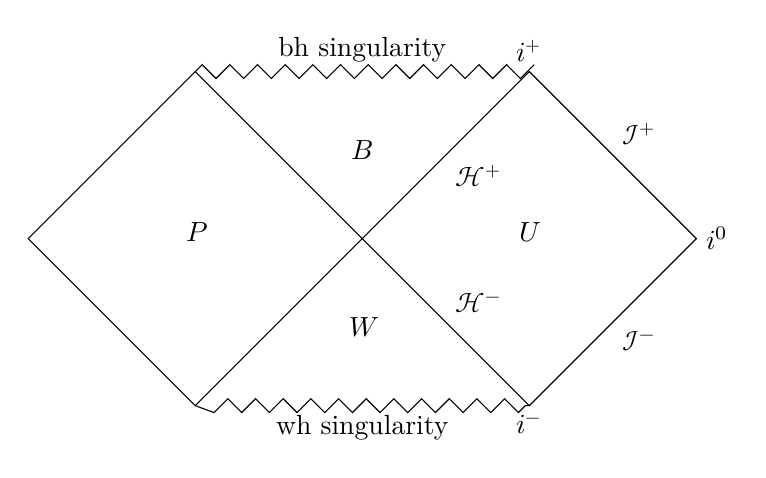
\begin{tikzpicture}%[scale=2]
\pgfmathsetmacro\myunit{3} 
	\draw (0,0)
			% node [left] {$i^0$} 
		--++(45:\myunit)
			% node [above]{$i^+$}
			coordinate (a)
			node [below = 1.8 cm] {$P$}
			% node [pos = .5, above left] {$\mscrI^+$}
			% node [pos=.5, below, sloped] {$\bar{u}=\infty$}
		--++(-45:2*\myunit)
			% node [pos = .25, above right] {$\mscrH^+$}
			node [pos = .75, above right] {$\mscrH^-$} %, sloped]{$r = \rSch$}%x_+ \to -\infty$}
			coordinate (d)	
			node [below]{$i^-$}
		--++(45:\myunit)
			node [pos = .5, below right] {$\mscrI^-$} % , sloped]{$x_- \to -\infty$}
			node [right] {$i^0$}
		--++(135:\myunit)
			node [pos = .5, above right] {$\mscrI^+$} % , sloped]{$x_+ \to +\infty$}
			node [above] {$i^+$}
			node [below = 1.8 cm] {$U$}
			coordinate (b)
		--++(-135:2*\myunit)
			coordinate (c)
			% node [pos = .25, below, sloped] {$r = \rSch$}%x_- \to +\infty$}
			% node [pos = .75, below right] {$\mscrH^-$}
			node [pos = .25, below right] {$\mscrH^+$}
			% node [below] {$i^-$}
		--cycle
			% node [pos = .5, below left] {$\mscrI^-$}
			;

	\draw [decorate, decoration=zigzag]
		(a) --
			node [above] {bh singularity} % =6pt
			node [below = .75 cm] {$B$}
			(b) 
		(c) --
			node [below] {wh singularity}
			node [above = .75 cm] {$W$}
			(d);

\end{tikzpicture}
\end{center}}
\only<2,4->{
\begin{itemize}
\item<4-> Comparing the space-time with that of the collapsing body:
\alert<4>{cut} along the dots and \alert<4>{stick} the right to an
interior solution
\item Clean calculation; $\abr{\what{\phi}^2}_\text{ren}$, 
$\abr{\what{T}_{\mu\nu}}_\text{ren}$ etc.\ obtainable
\item Different `vacua' can be defined
\begin{itemize}
\item \alert<2>{Boulware}: No flux, $\abr{\what{\phi}^2}_\text{ren}$
blows up at $\mscrH^-\cup\mscrH^+$
	\begin{itemize}
	\item<2> Miracle near the horizons
	\end{itemize}
\item \alert<2>{Israel--Hartle--Hawking}: I/O flux,
$\abr{\what{\phi}^2}_\text{ren}$ finite at $\mscrH^-\cup\mscrH^+$
	\begin{itemize}
	\item<2> Black hole in a heat bath
	\item<2> \alert<2>{Mathematically} more desirable
	\end{itemize}
\item \alert<2,4>{Unruh}: O flux, $\abr{\what{\phi}^2}_\text{ren}$
blows up at $\mscrH^-$
	\begin{itemize}
	\item<4> $\mscrH^-$ and the divergence therein can be hidden
	\item<4> Similar to the (physical) collapsing case
	\end{itemize}
\end{itemize}
\end{itemize}}
\only<3>{
\begin{center}
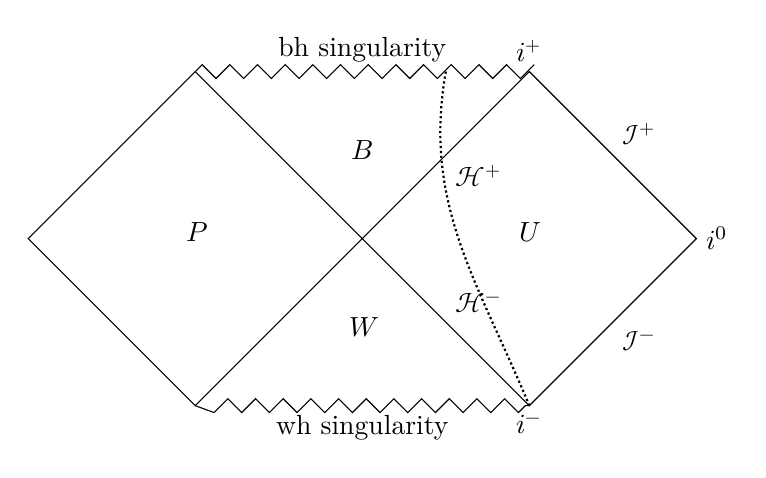
\begin{tikzpicture}%[scale=2]
\pgfmathsetmacro\myunit{3} 
	\draw (0,0)
			% node [left] {$i^0$} 
		--++(45:\myunit)
			% node [above]{$i^+$}
			coordinate (a)
			node [below = 1.8 cm] {$P$}
			% node [pos = .5, above left] {$\mscrI^+$}
			% node [pos=.5, below, sloped] {$\bar{u}=\infty$}
		--++(-45:2*\myunit)
			% node [pos = .25, above right] {$\mscrH^+$}
			node [pos = .75, above right] {$\mscrH^-$} %, sloped]{$r = \rSch$}%x_+ \to -\infty$}
			coordinate (d)	
			node [below]{$i^-$}
		--++(45:\myunit)
			node [pos = .5, below right] {$\mscrI^-$} % , sloped]{$x_- \to -\infty$}
			node [right] {$i^0$}
		--++(135:\myunit)
			node [pos = .5, above right] {$\mscrI^+$} % , sloped]{$x_+ \to +\infty$}
			node [above] {$i^+$}
			node [below = 1.8 cm] {$U$}
			coordinate (b)
		--++(-135:2*\myunit)
			coordinate (c)
			% node [pos = .25, below, sloped] {$r = \rSch$}%x_- \to +\infty$}
			% node [pos = .75, below right] {$\mscrH^-$}
			node [pos = .25, below right] {$\mscrH^+$}
			% node [below] {$i^-$}
		--cycle
			% node [pos = .5, below left] {$\mscrI^-$}
			;

	\draw [decorate, decoration=zigzag]
		(a) --
			node [above] {bh singularity} % =6pt
			node [below = .75 cm] {$B$}
			(b) 
		(c) --
			node [below] {wh singularity}
			node [above = .75 cm] {$W$}
			(d);

	\draw [thick, densely dotted, out = 112.5, in = -100] (d)
		to ($(a)!0.75!(b)$);
\end{tikzpicture}
\end{center}}
\end{frame}

%\item Wave-functional formalisms
%	\begin{itemize}
%	\item Painlevé and Lemaı̂tre coordinates
%	\item Same physics as in ...
%	\end{itemize}
%\item Canonical quantum gravitation 


%\begin{frame}{Canonical quantum gravitation}{In toy gravitation models}
%\cite{Callan1992}
%\begin{itemize}
%	\item QFT in CST recovered in Born-Oppenheimer expansion \cite{Demers1996}
%\end{itemize}

%\end{frame}


\section{Information loss problem}

\begin{frame}{Information loss problem}{See e.g.\ 
\cite{Mathur2009,Mann2015}}%{Grey-body radiation from black holes}
\begin{columns}
\begin{column}{.61\textwidth}
\begin{itemize}
\item Minkowski: particles from $\mscrI^-$ to $\mscrI^+$
\item<2-> Collapsing body: can also go to $\mscrH^+$
\item<2-> Obs.\ able to set up \alert<2>{input} at $\mscrI^-$ and
collect \alert<2>{output} at $\mscrI^+$, but \alert<2>{not} at $\mscrH^+$
\item<3-> $\Ket{\alpha}$ on $\mscrI^-$ evolves to $\Ket{\beta}$ on $\mscrH^+ 
\cup \mscrI^+$
\item<3-> \alert<3>{Pure} $\what{\rho}_\text{I} = \Ket{\alpha}\Bra{\alpha}$
turns \alert<3>{mixed} $\what{\rho}_\text{O} = \mathrm{tr}_{\mscrH^+}
\Ket{\beta}\Bra{\beta}$! Something is lost
\item<4-> Non-conservation arguments \cite{Hawking1976}
\item<4-> Conservation arguments \cite{Page1993}
\end{itemize}
\end{column}
\begin{column}[c]{.38\textwidth}
\only<1>{
\begin{tikzpicture}%[scale=2]
\pgfmathsetmacro\myunit{3} 
	\draw (0,0)
			node [above] {$i^+$}
		--++(-45:\myunit)
			node [right] {$i^0$}
			node [pos = .5, above right] {$\mscrI^+$}
		--++(-135:\myunit)
			coordinate (b)
			node [below] {$i^-$}
			node [pos = .5, below right] {$\mscrI^-$};
	\draw [dashed] (b) -- (0,0);
\end{tikzpicture}}
\only<2->{
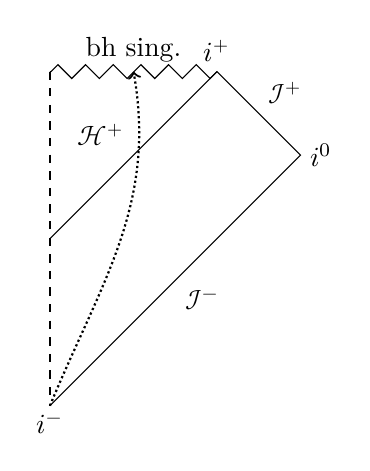
\begin{tikzpicture}%[scale=2]
\pgfmathsetmacro\myunit{3} 
\pgfmathsetmacro\sc{1.414213562} 
	\draw [dashed] (0,0)
		-- ++(-90: \sc * \myunit)
			node [below] {$i^-$}
			coordinate (a);
	\draw (a)
		-- ++(45: 1.5 * \myunit)
			node [right] {$i^0$}
			node [pos = .5, below right] {$\mscrI^-$}
		-- ++(135: 0.5 * \myunit)
			node [above] {$i^+$}
			node [pos = .5, above right] {$\mscrI^+$}
			coordinate (b)
		-- ++(-135: \myunit)
			node [pos = .5, above left] {$\mscrH^+$};
	\draw [decorate, decoration=zigzag] (b)
		-- (0,0)
			node [pos = .5, above] {bh sing.};
	\draw [densely dotted, out = 67.5, in = -80, thick, ->] (a)
			to (\sc/4* \myunit, 0);
\end{tikzpicture}}
\end{column}
\end{columns}
\end{frame}

%\begin{frame}{Interpretations}%{Grey-body radiation from black holes}
%\begin{itemize}
%\item Thermal-like radiation
%	\begin{itemize}
%	\item 123
%	\end{itemize}

%\item Entropies and temperatures
%\item Progressive evaporation
%\item Final fate
%\item Information
%	\begin{itemize}
%	\item Non-conservation \cite{Hawking1976}
%	\item Conservation \cite{Page1993}
%	\end{itemize}
%\item Violation of unitarity
%\end{itemize}

%\end{frame}


%\section{Questions}
%\begin{frame}{Questions}
%\begin{itemize}
%\item Field, not gravitation itself
%\item Thermality of the radiation
%\end{itemize}

%\end{frame}


\section*{Summary}

\begin{frame}{Summary}

  % Keep the summary *very short*.
  \begin{itemize}
  \item
    \alert{Robust} calculation of outgoing particle flux for the space-time
	of collapsing body
  \item
    \alert{Controversial} interpretations and extrapolations
  %\item
    %Perhaps a \alert{third message}, but not more than that.
  \end{itemize}
  \vskip0pt plus.5fill
  \begin{itemize}
  \item Back-reaction to the metric: no time
  \end{itemize}  
  % The following outlook is optional.
  \vskip0pt plus.5fill
  \begin{itemize}
  \item
    Seeks combination with
    \begin{itemize}
    \item Quantum gravitation
    \item Quantum information
	%\item Super-string theory
    \end{itemize}
  \end{itemize}
\end{frame}



% All of the following is optional and typically not needed. 
\appendix
%\section<presentation>*{\appendixname}
%\subsection<presentation>*{For Further Reading}

\begin{frame}[allowframebreaks]
  \frametitle<presentation>{References}
%\printbibliography
    
%  \begin{thebibliography}{10}
    
  \beamertemplatebookbibitems
  % Start with overview books.
\printbibliography[type=book]

%  \bibitem{Author1990}
%    A.~Author.
%    \newblock {\em Handbook of Everything}.
%    \newblock Some Press, 1990.
 
    
  \beamertemplatearticlebibitems
  % Followed by interesting articles. Keep the list short. 
\printbibliography[nottype=book]

%  \bibitem{Someone2000}
%    S.~Someone.
%    \newblock On this and that.
%    \newblock {\em Journal of This and That}, 2(1):50--100,
%    2000.
%  \end{thebibliography}
\end{frame}



\end{document}
